% ------------------------------------------------------------------
% Fig. 1 -- System architecture.
%
% Drawn in the visual idiom of the tikz.net machine-learning diagrams
% (tikz.net/category/computing/machine-learning): a standalone
% document, grayscale fills, bold stage captions set outside the
% nodes, and chunky grey arrows carrying the stage-to-stage flow --
% black and white throughout, no color, per print-format requirement.
%
% Strictly left to right -- no cycles. The search loop is Fig. 2.
% Compile on its own:  tectonic -X compile figures/fig_architecture.tex
% ------------------------------------------------------------------
\documentclass[tikz,border=5pt]{standalone}
\usepackage{amsmath,amssymb}
\usetikzlibrary{positioning,arrows.meta,calc,fit}

\begin{document}
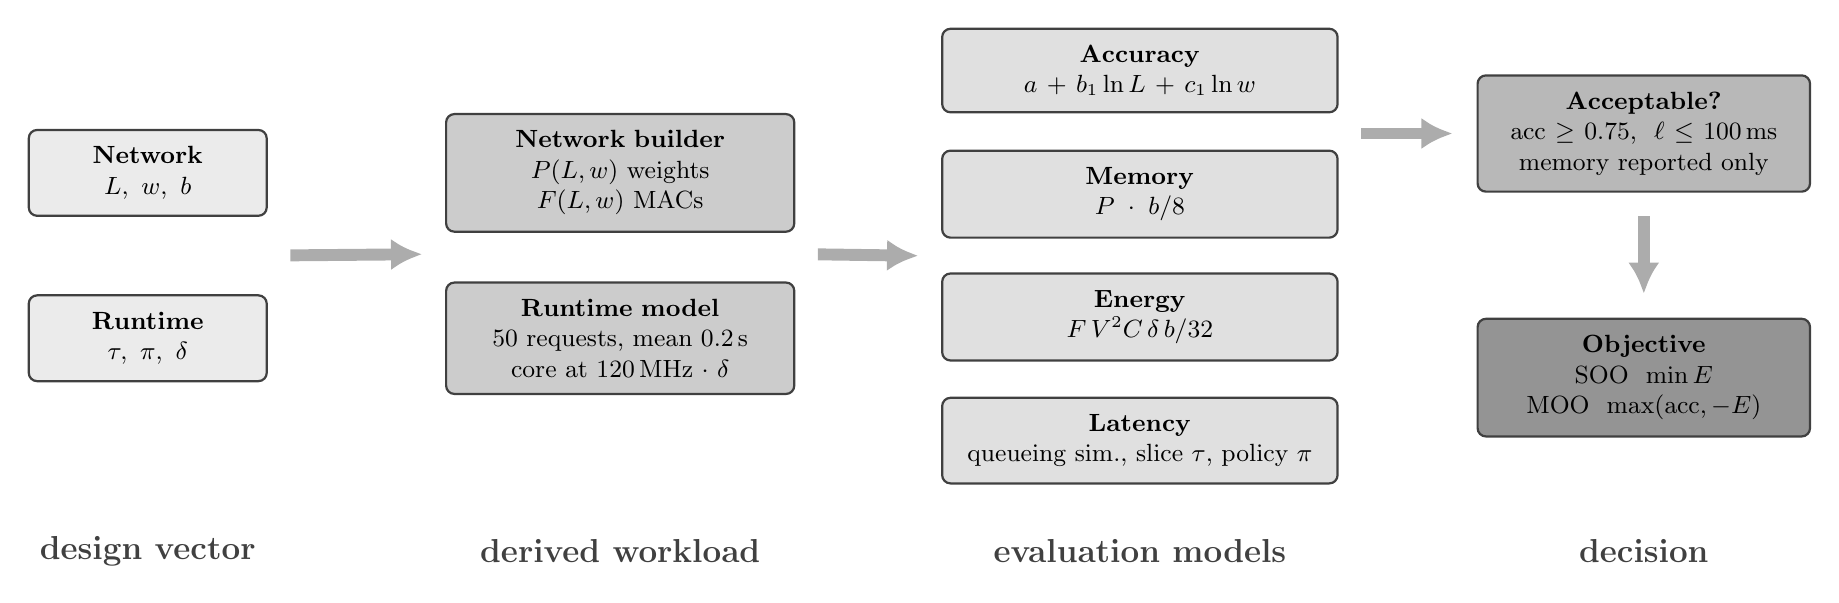
\begin{tikzpicture}[
    thick,
    font=\small,
    blk/.style   = {rounded corners=3pt, draw=black!75, align=center,
                    inner sep=6pt},
    inp/.style   = {blk, fill=black!8,   text width=26mm},
    drv/.style   = {blk, fill=black!20,  text width=40mm},
    mdl/.style   = {blk, fill=black!12,  text width=46mm},
    gate/.style  = {blk, fill=black!28,  text width=38mm},
    obj/.style   = {blk, fill=black!42,  text width=38mm},
    stage/.style = {font=\large\bfseries, text=black!75},
    arrow/.style = {>={LaTeX[width=4mm,length=4mm]}, ->, line width=1ex,
                    gray!65, shorten <=3mm, shorten >=3mm},
  ]

% ---------- stage 1: the design vector ------------------------------
\begin{scope}[local bounding box=A]
  \node[inp] (net) at (0, 1.05)  {\textbf{Network}\\ $L,\ w,\ b$};
  \node[inp] (rt)  at (0,-1.05)  {\textbf{Runtime}\\ $\tau,\ \pi,\ \delta$};
\end{scope}

% ---------- stage 2: derived workload -------------------------------
\begin{scope}[local bounding box=B]
  \node[drv] (build) at (6.0, 1.05)
       {\textbf{Network builder}\\ $P(L,w)$ weights\\ $F(L,w)$ MACs};
  \node[drv] (req)   at (6.0,-1.05)
       {\textbf{Runtime model}\\ 50 requests, mean $0.2$\,s\\
        core at $120\,\mathrm{MHz}\cdot\delta$};
\end{scope}

% ---------- stage 3: the four evaluation models ---------------------
\begin{scope}[local bounding box=C]
  \node[mdl] (acc) at (12.6, 2.35) {\textbf{Accuracy}\\ $a+b_1\ln L+c_1\ln w$};
  \node[mdl] (mem) at (12.6, 0.78) {\textbf{Memory}\\ $P\cdot b/8$};
  \node[mdl] (en)  at (12.6,-0.78) {\textbf{Energy}\\ $F\,V^{2}C\,\delta\,b/32$};
  \node[mdl] (lat) at (12.6,-2.35) {\textbf{Latency}\\ queueing sim.,
        slice $\tau$, policy $\pi$};
\end{scope}

% ---------- stage 4: acceptability, then objective ------------------
\begin{scope}[local bounding box=D]
  \node[gate] (g) at (19.0, 1.55)
       {\textbf{Acceptable?}\\ $\mathrm{acc}\geq0.75$,\ \ $\ell\leq100$\,ms\\
        memory reported only};
  \node[obj]  (o) at (19.0,-1.55)
       {\textbf{Objective}\\ SOO\ \ $\min E$\\ MOO\ \ $\max(\mathrm{acc},-E)$};
\end{scope}
\draw[arrow] (g) -- (o);

% ---------- the flow ------------------------------------------------
\draw[arrow] (A.east) -- (B.west);
\draw[arrow] (B.east) -- (C.west);
\draw[arrow] (C.east |- g.west) -- (g.west);

% ---------- stage captions ------------------------------------------
\node[stage] at (0,   -3.75) {design vector};
\node[stage] at (6.0, -3.75) {derived workload};
\node[stage] at (12.6,-3.75) {evaluation models};
\node[stage] at (19.0,-3.75) {decision};

\end{tikzpicture}
\end{document}
